% Drawing 74/07-2 -- folder 74, batch 07, archive page 124 (PDF page 125).
% Transcription: trois ovales reliés, contenant $\xi_1\ \xi_2\ \xi_3$ / $\xi_4^*\ \xi_5^*\ \xi_6^*$ ; $\xi_4\ \xi_5\ \xi_6$ / $\xi_1'\ \xi_2'\ \xi_3'$ ; $\xi_{45}\ \xi_{56}\ \xi_{64}$ / $\xi_{12}\ \xi_{23}\ \xi_{31}$.
% Kind: three linked ovals of symbols. Method 2 (schematic redraw from the facsimile). Status: ok.
% Notes: Three ovals in thin ink: the top one with xi45 xi56 xi64 / xi12 xi23 xi31, the lower left one with xi1 xi2 xi3 / xi4* xi5* xi6*, the lower right one with xi4 xi5 xi6 / xi1' xi2' xi3' (contents as the transcription reads them, each symbol where it is written; the first symbols of the two rows of the top oval are overwritten with a star). The top and lower left ovals are closed; the lower right one is open at the lower right, its left side running down into a loop under it. Links: a short stroke joins the two lower ovals at the height of their first rows, a second one at the bottom joins the lower left oval to the loop under the lower right one, a thin oblique stroke runs from the bottom of the top oval to xi6* in the lower left one, and a long curve leaves the top oval beside xi64 and runs down along the right side of the lower right oval. Struck out and omitted: the scribbles crossing out a group of symbols at the left of the top oval (the symbols under them are text, not read), and the zigzags at the far left. Overlay check 2026-11-13 (issue 147, Claude claude-opus-5-5): the redraw, rasterised by the skill's previewer (not compiled: no TeX in the session), laid over the 300 dpi colour crop of the scan (261 ppi). The earlier redraw's ovals were smooth closed curves 2 to 5 units off the page's (the lower right one closed where the page's is open), with the contents set as three-symbol rows and only one linking stroke: the ovals are redrawn through points read on their ink, each symbol is set where it is written, and the second bottom stroke, the oblique stroke and the long curve at the right are added. Matches the facsimile.
% Coordinates: 1 unit = 1 mm = 1/100 of the crop width (bbox in page fractions: [0.06, 0.38, 0.45, 0.62]).
% Redrawn by Claude (claude-opus-5-5), issue #73, 2026-11-09; not checked by a human; not compiled (no TeX in the session).
% Checked by Claude (claude-opus-5-5) 2026-11-13 (issue #147): overlaid on the 300 dpi colour facsimile and corrected; not compiled (no TeX in the session). Status: ok.
% Rights: reproduces part of the work -- behind RENDER_TRANSCRIPTS, never published by itself.
\documentclass[tikz,border=3pt]{standalone}
\usepackage{amsmath,amssymb}
\usetikzlibrary{patterns,arrows.meta}
\tikzset{pencil/.style={black!45}, struck/.style={black!35}, mark/.style={circle,draw,inner sep=1.3pt}, pt/.style={circle,fill,inner sep=0.9pt}, opt/.style={circle,draw,fill=white,inner sep=1.1pt}}
\begin{document}
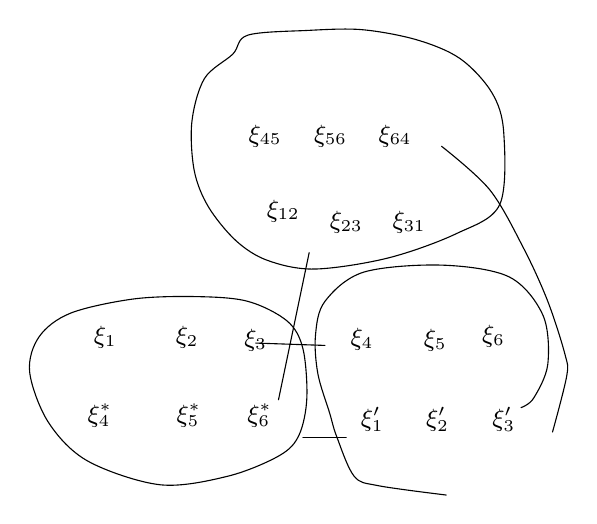
\begin{tikzpicture}[x=1mm,y=1mm,line cap=round,line join=round,font=\scriptsize]
\draw plot[smooth cycle, tension=0.55] coordinates {(44.5,-24.2) (52,-23.6) (59,-23.5) (66,-24.8) (71.5,-27.2) (75.5,-31.5) (77,-36.5) (76.5,-45.7) (71,-49.4) (62.3,-52.5) (53,-53.9) (47,-52.8) (43,-50.3) (39.5,-46) (37.7,-41.4) (37.4,-35.2) (39,-29.7) (42.6,-26.6)};
\draw plot[smooth cycle, tension=0.55] coordinates {(22,-59.5) (30,-57.7) (38,-57.4) (44.5,-58) (49.5,-60.5) (51.5,-64) (52,-70.3) (51,-75) (48.5,-77.6) (42,-80.2) (33.4,-81.3) (24.2,-78.3) (19.2,-73.4) (16.8,-67) (18,-62.5)};
\draw plot[smooth, tension=0.55] coordinates {(79.2,-71.5) (80.8,-70.3) (82.6,-66) (82,-59.8) (77.7,-54.9) (69.1,-53.4) (59.2,-54.3) (54.3,-58) (53.1,-62.3) (53.4,-67.2) (54.9,-72.2) (55.8,-75.2) (58,-80.2) (61,-81.4) (69.7,-82.6)};
\draw plot[smooth, tension=0.55] coordinates {(69.1,-38.3) (75.2,-43.8) (79.5,-51.2) (82.6,-58) (84.8,-64.8) (85,-67.5) (83.2,-74.6)};
\draw (45.5,-63.3) -- (54.3,-63.6);
\draw (51.5,-75.3) -- (57,-75.3);
\draw (52.3,-51.8) -- (48.4,-70.5);
\node[inner sep=1pt] at (46.7,-37) {\small $\xi_{45}$};
\node[inner sep=1pt] at (55,-37) {\small $\xi_{56}$};
\node[inner sep=1pt] at (63.2,-37) {\small $\xi_{64}$};
\node[inner sep=1pt] at (49,-46.5) {\small $\xi_{12}$};
\node[inner sep=1pt] at (57,-48) {\small $\xi_{23}$};
\node[inner sep=1pt] at (65,-48) {\small $\xi_{31}$};
\node[inner sep=1pt] at (26.4,-62.6) {\small $\xi_1$};
\node[inner sep=1pt] at (36.8,-62.6) {\small $\xi_2$};
\node[inner sep=1pt] at (45.5,-63) {\small $\xi_3$};
\node[inner sep=1pt] at (25.7,-72.5) {\small $\xi_4^*$};
\node[inner sep=1pt] at (37,-72.5) {\small $\xi_5^*$};
\node[inner sep=1pt] at (46,-72.5) {\small $\xi_6^*$};
\node[inner sep=1pt] at (59,-62.8) {\small $\xi_4$};
\node[inner sep=1pt] at (68.3,-63) {\small $\xi_5$};
\node[inner sep=1pt] at (75.7,-62.5) {\small $\xi_6$};
\node[inner sep=1pt] at (60.3,-73) {\small $\xi_1'$};
\node[inner sep=1pt] at (68.6,-73) {\small $\xi_2'$};
\node[inner sep=1pt] at (77,-73) {\small $\xi_3'$};
\end{tikzpicture}
\end{document}
